% Created 2022-10-13 Thu 23:01
% Intended LaTeX compiler: pdflatex
\documentclass[11pt]{article}
\usepackage[utf8]{inputenc}
\usepackage[T1]{fontenc}
\usepackage{graphicx}
\usepackage{float} % used to cancel the automatic table positioning , use [H] for here.
\usepackage{grffile}
\usepackage{longtable}
\usepackage{wrapfig}
\usepackage{rotating}
\usepackage[normalem]{ulem}
\usepackage{amsmath}
\usepackage{textcomp}
\usepackage{amssymb}
\usepackage{capt-of}
\usepackage{hyperref}
\usepackage{parskip}
\usepackage{tabularx}

\author{Omkar Girish Kamath}
\date{\today}
\title{Specification Document}
\hypersetup{
  pdfauthor={Omkar Girish Kamath},
  pdftitle={Specification Document},
  pdfkeywords={},
  pdfsubject={},
  pdfcreator={Emacs 26.3 (Org mode 9.1.9)}, 
  pdflang={English}}
\begin{document}

\maketitle
\tableofcontents
\vspace*{40mm}
\section{Processor}
\begin{figure}[!h]
  \begin{center}
    \caption{}
    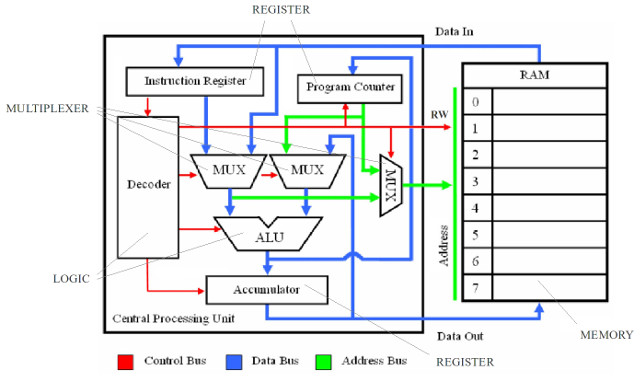
\includegraphics[scale=0.5]{top_view.jpg}
  \end{center}
\end{figure}
\subsection{Major Modules and Their Functions}
\subsubsection{Program Counter}
Program Counter (PC) : 8 bit register used to store the address in memory of the current instruction being executed.
\subsubsection{Instruction Register}
Instruction Register (IR) : 16 bit register, updated at the end of the fetch phase with the instruction to be processed (decoded and executed).
\subsubsection{Accumulator }
8 bit register, a general purpose data register, providing data (operand) to be processed by the ALU and used to store any result produced. Note, we can only store one 8 bit value at a time on the processor, other data values will need to be buffered in external memory.
\subsubsection{Decoder}
It decodes the 16 bit instruction recieved , tracks the state of the processor and generates control signals based on the first two.
\subsubsection{ALU}
It is the arithmetic and logic unit , which can take in 1 or 2 8bit inputs and perform arithmetic and logic based operations on the operand. 
\subsection{Instruction Set}
\label{sec:org4f08230}

In this instruction syntax X=Not used, K=Constant, A=Instruction Address, P=Data Address

\begin{longtable}{|l|l|l|}
  \caption{Instruction Set of the Simple CPU}\\ \hline
          {\bf Opcode} & {\bf Instruction} & {\bf RTL} \\ 
          \endfirsthead
          \caption[]{(\em continued from previous page)}\\
          \hline
              {\bf Opcode} & {\bf Instruction} & {\bf RTL} \\ \hline 
              \endhead
              \multicolumn{3}{|r|}{{\em continued on next page}} \\ \hline
              \endfoot
              \endlastfoot
              \hline \hline
              \texttt{Load ACC kk} &  \texttt{0000 XXXX KKKKKKKK} & \texttt{ACC <- KK} \\ \hline
              
              \texttt{Add ACC kk} &  \texttt{0100 XXXX KKKKKKKK} & \texttt{ACC <- ACC + KK} \\ \hline
              
              \texttt{And ACC kk} &  \texttt{0001 XXXX KKKKKKKK} &  \texttt{ACC <- ACC \& KK} \\ \hline
              
              \texttt{Sub ACC kk} &  \texttt{0110 XXXX KKKKKKKK} & \texttt{ACC <- ACC - KK} \\ \hline
              
              \texttt{Input ACC pp} &  \texttt{1010 XXXX PPPPPPPP} & \texttt{ACC <- M[PP]} \\ \hline
              
              \texttt{Output ACC pp} &  \texttt{1110 XXXX PPPPPPPP} & \texttt{M[PP] <- ACC} \\ \hline
              
              \texttt{Jump U aa} &  \texttt{1000 XXXX AAAAAAAA} & \texttt{PC <- AA} \\ \hline
              
              \texttt{Jump Z aa} &  \texttt{1001 00XX AAAAAAAA} & \texttt{IF Z=1 PC <- AA ELSE PC <- PC + 1} \\ \hline
              
              \texttt{Jump C aa} &  \texttt{1001 10XX AAAAAAAA} & \texttt{IF C=1 PC <- AA ELSE PC <- PC + 1} \\ \hline
              
              \texttt{Jump NZ aa} &  \texttt{1001 01XX AAAAAAAA} & \texttt{IF Z=0 PC <- AA ELSE PC <- PC + 1} \\ \hline
              
              \texttt{Jump NC aa} &  \texttt{1001 11XX AAAAAAAA} & \texttt{IF C=0 PC <- AA ELSE PC <- PC + 1}\\ \hline
              
\end{longtable}


Here '->' indicates updated with .

The processor has an extra cycle to save on hardware which would have been required for incrementing the PC . So the processor follows \textbf{fetch-decode-execute-increment} cycle .
THe processor uses a 1 GHz frequency clock.

\subsection{Functioning of the processor}
\begin{figure}[H]
  \begin{center}
    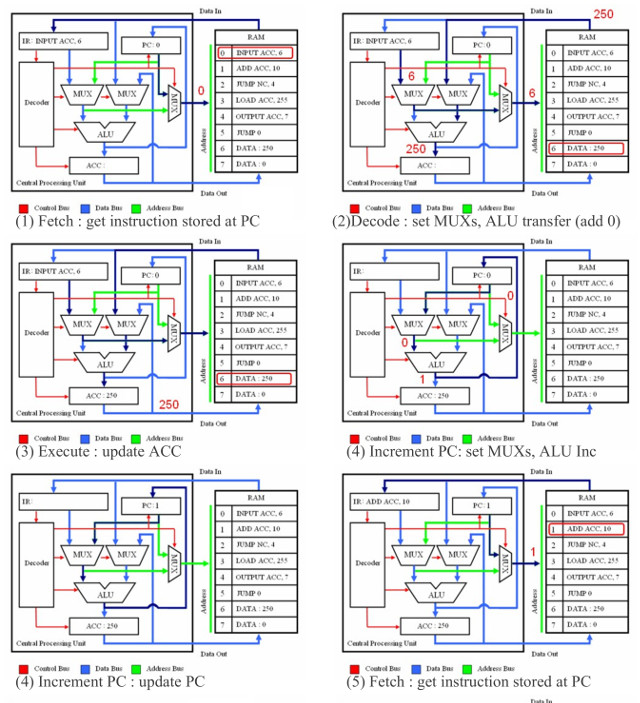
\includegraphics[scale=0.5]{steps_1_to_5_tmb.jpg}
  \end{center}
\end{figure}

\textbf{ Step 1} : reset, clear line pulsed to reset all flip-flop, initialising all registers to their default values. First fetch phases initiated, ADDR MUX selects PC i.e. the value 0, memory address 0 read, first instruction (INPUT) stored in IR. \\
\textbf{Step 2} : decode, opcode field decoded, instruction identified as an INPUT instruction, control-logic configures data paths to route absolute address (6) stored in IR to address bus using ADDR MUX. Memory read, data at address 6 accessed (250), data driven onto data-in bus, routed through DATA MUX to input of ACC.\\
\textbf{Step 3} : execute, ACC updated with accessed data, at the end of this phase ACC = 250. \\
\textbf{Step 4} : increment, instruction completed, processor needs to increment PC to the address of the next instruction. Control-logic configures ALU to perform increment function, PC routed to ALU, value incremented and stored back into PC. \\ 
\textbf{Step 5} : fetch, instruction at address 1 read (ADD) and stored in IR. \\
\subsection{Input Output Interface}
\begin{table}[H]
  \begin{center}
    \caption{I/O interface of the processor}  
    \vspace*{5mm}
    \begin{tabularx}{\linewidth}{||l|l|l||l|X||}
      \hline
          {\bf Signals} & { \bf Type } & {\bf Size} & {\bf Active} &{\bf Description}   \\ \hline
            clk          & input  & 1 bit   & -     &  square wave used to maintain synchronousity in the device \\ \hline
            rst          & input  & 1 bit   & Low   &  resets the chip to a pre decided state \\ \hline
            [15:0] d\_in & input  & 16 bits & -     &  the instruction sent from memory \\ \hline
            [7:0] adrs   & output & 8 bits  & -     &  the address of the required instruction sent to memory \\ \hline
            rw           & output & 1 bit   & -     &  read write control signal sent to memory \\ \hline
            [7:0] d\_out & output & 8 bits  & -     &  output data from the processor \\ \hline
    \end{tabularx}
  \end{center}
\end{table}
\subsection{Timing Diagrams}
\begin{figure}[!h]
  \caption{Timing Diagrams of the processor}
  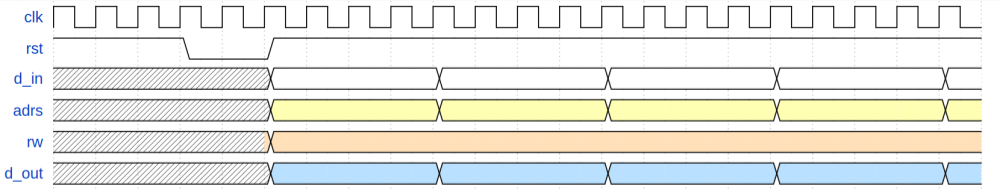
\includegraphics[scale=0.4]{./images/MergedImages.png}
\end{figure}
\section{Memory}
\subsection{Description}
{\bf Size of RAM -> 4 Kilobytes} \\
RAM used is Volatile BJT type Synchronous Static RAM . \\
Instruction length is \textit{16 bit} , maximum number of instructions  and data than can be stored is {\bf 256} (address 0 to 255).
Address length required is 8 bits.
\subsection{I/O of the  Memory device}

\begin{table}[H]
  \begin{center}
    \caption{I/O of the Memory device}
    \begin{tabularx}{\linewidth}{||l|l|l|l|X||}
      \hline
      {\bf Signals} & { \bf Type } & {\bf Size} & {\bf Active} &{\bf Description}   \\ \hline
            clk            & input  & 1 bit   & -     &  square wave used to maintain synchronousity in the device \\ \hline
            rst            & input  & 1 bit   & Low   &  resets the memory to a pre decided state \\ \hline
            [15:0] mem\_in & input  & 16 bits & -     &  the data sent by chip \\ \hline
            [7:0] adrs     & input  & 8 bits  & -     &  the address of the required instruction \\ \hline
            rw             & input  & 1 bit   & -     &  read write control signal sent to memory \\ \hline
            [15:0] mem\_out& output & 16 bits & -     &  output data/instruction from the memory \\ \hline
    \end{tabularx}
  \end{center}
\end{table}
\end{document}
